\chapter{Case Study Baseline (As-Is System)}
\label{chap:baseline}

This chapter describes the initial state of Outsight Cloud before the migration strategy was formalized, establishing the architectural and operational baseline against which migration decisions are evaluated.

\section{Current Architecture and Data Flow}
Before the migration to AWS, Outsight Cloud relied on a containerized architecture designed for rapid feature delivery. The platform managed LiDAR-related workflows and assets through a web application and backend API stack composed of several interconnected components: a \textbf{Vue 3 SPA frontend}; a \textbf{Node.js/Express backend API} implementing business logic and integrations; \textbf{Redis} for session management; \textbf{Docker Compose} orchestrating containers on \textbf{DigitalOcean Droplets}; a \textbf{Traefik} reverse proxy for HTTPS termination and routing; \textbf{Airtable} as the primary operational datastore for users, organizations, sites, simulations, and permissions; \textbf{S3-compatible object storage} for simulation files; \textbf{GitBook} for documentation; and \textbf{Slack and Customer.io} integrations for notifications.

From an infrastructure perspective, the architecture followed a virtual-machine-centric model in which scaling, upgrades, deployment, and maintenance were handled directly by the engineering team. While sufficient during the early stages, this approach increasingly exposed limitations related to scalability, operational governance, fault tolerance, and infrastructure reproducibility.

\begin{figure}[htbp]
    \centering
    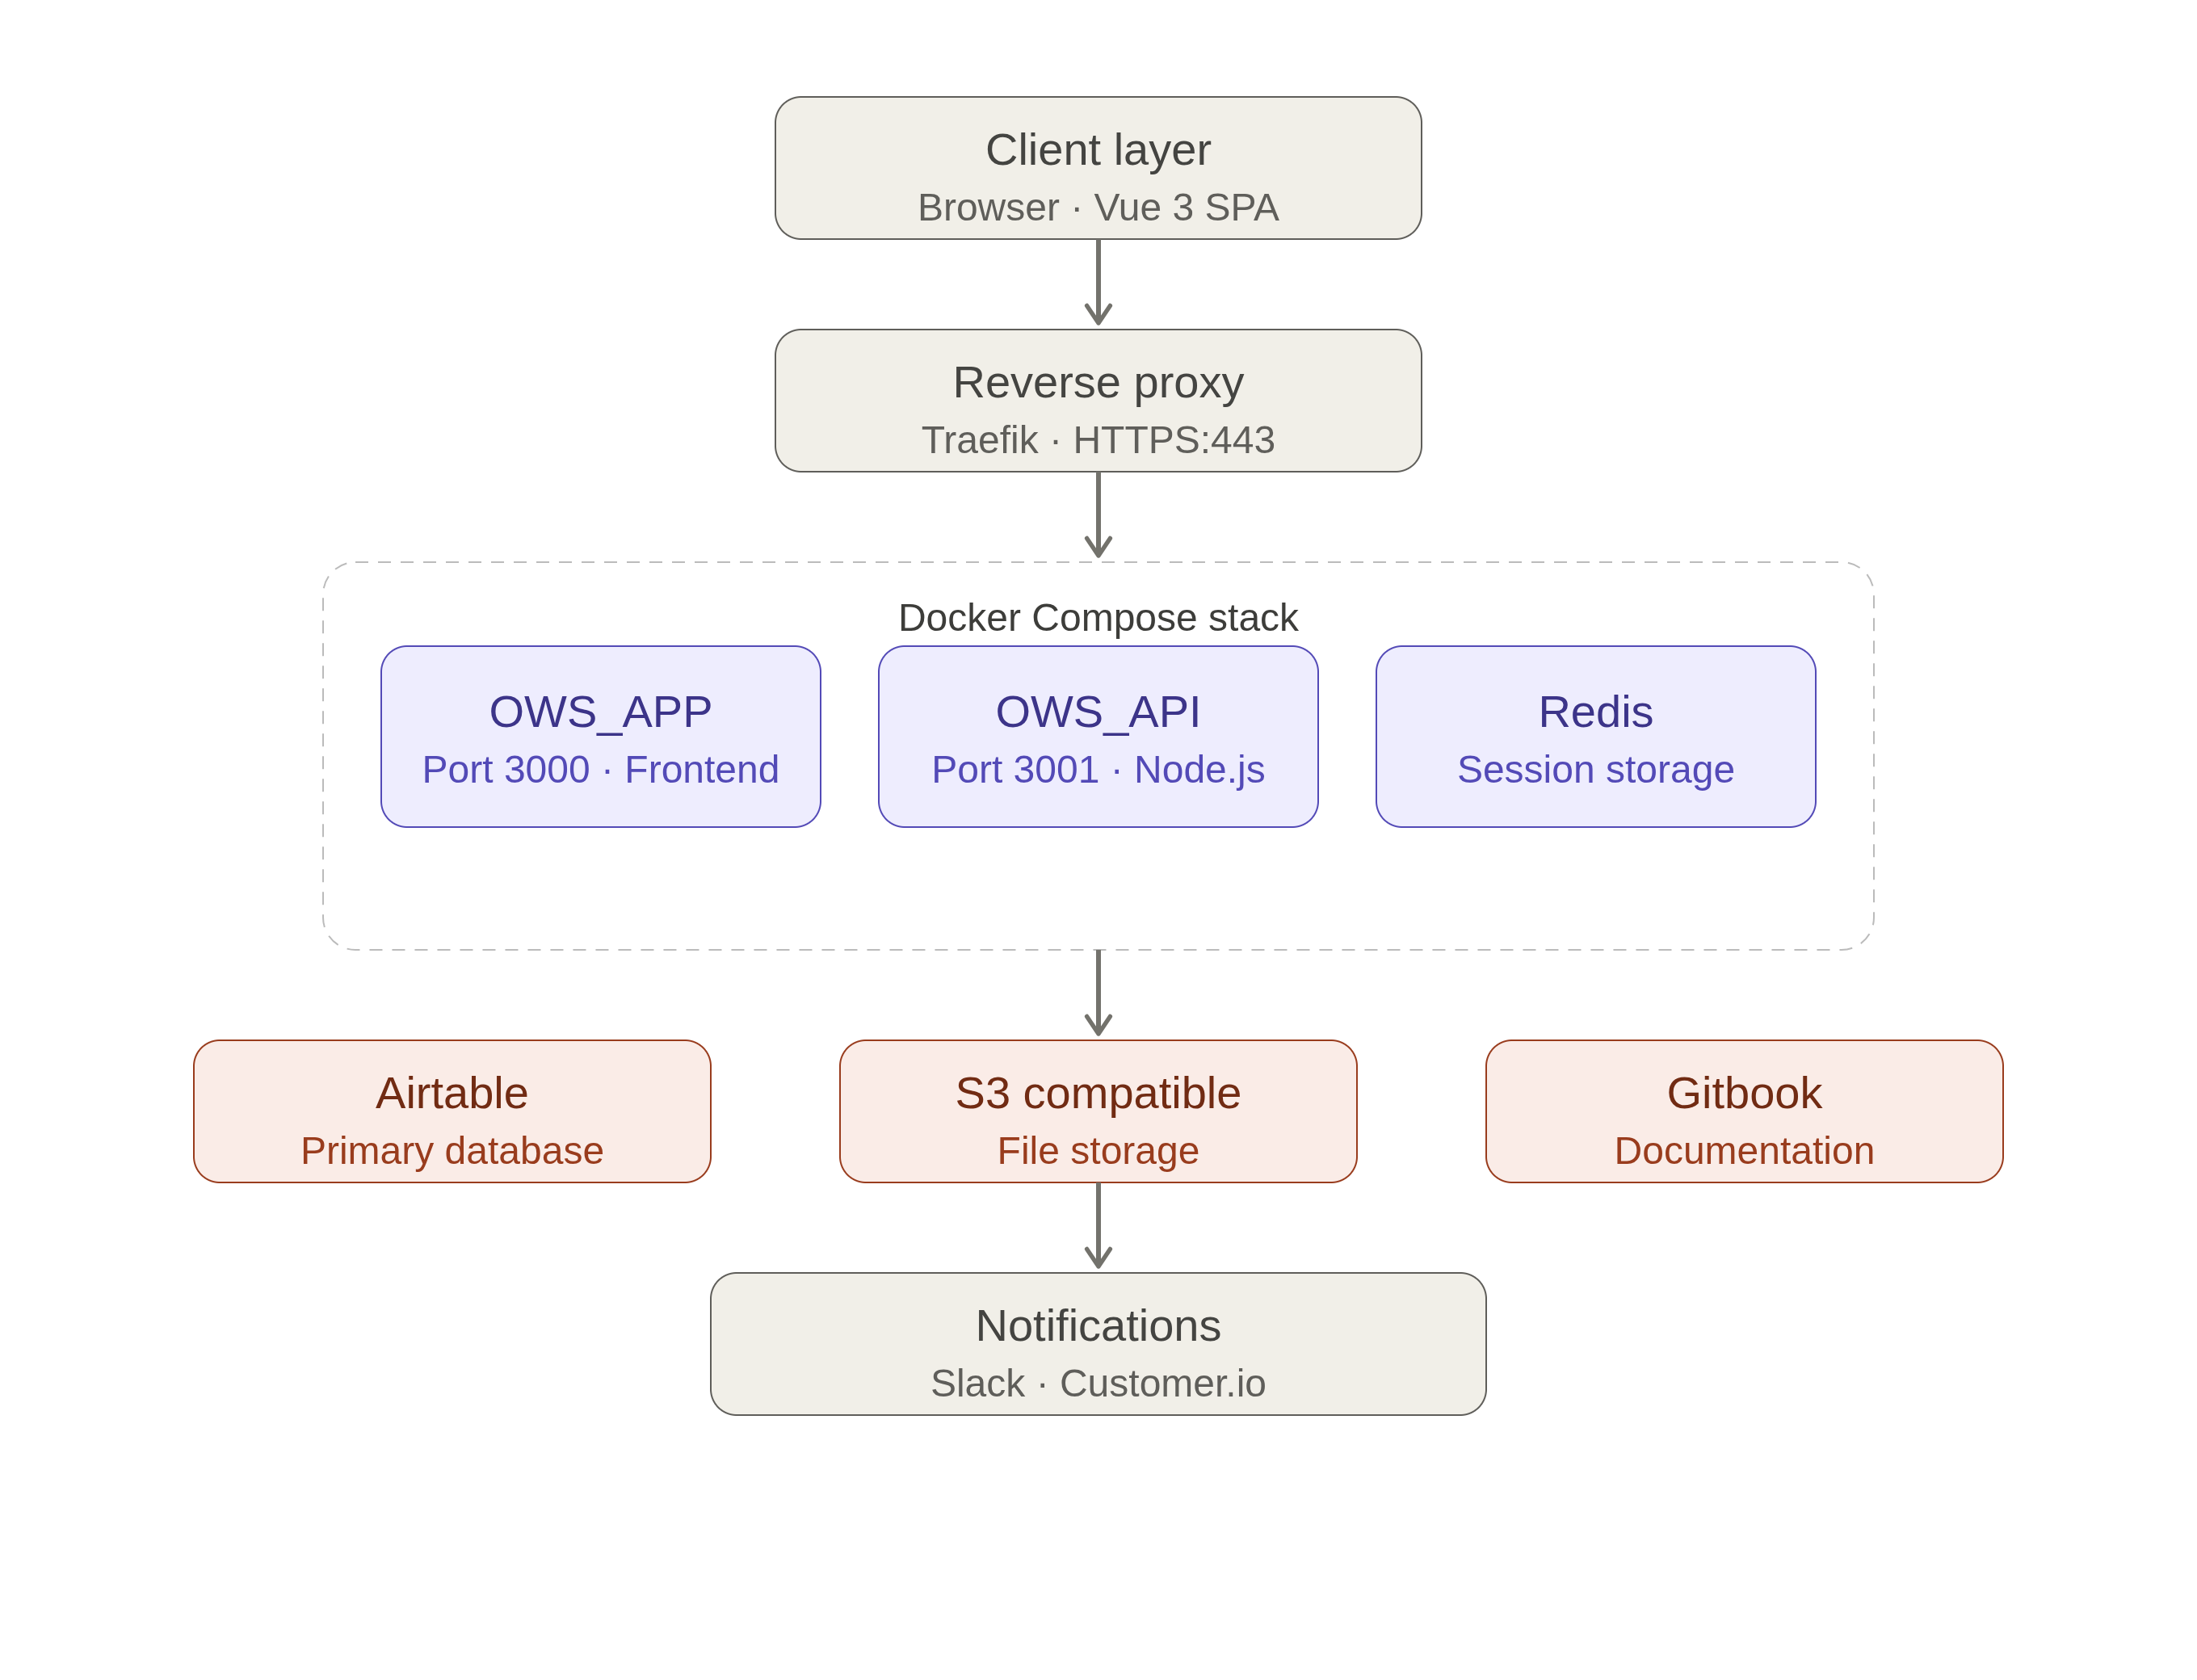
\includegraphics[width=0.95\textwidth]{immagini/outsight_legacy_architecture.png}
    \caption{Outsight Cloud baseline architecture before the migration.}
    \label{fig:outsight-as-is-architecture}
\end{figure}

\section{Airtable as Primary Data Storage}
Airtable was more than a persistence layer: it acted simultaneously as operational datastore, workflow-management layer, and integration hub. Airtable is a cloud-based platform combining spreadsheet-like interfaces with lightweight database capabilities, organizing data into bases, tables, records, and fields, and providing views, forms, automations, and API access~\cite{airtableBasics}. In Outsight Cloud these capabilities were exercised through API access, operational forms, and integrations such as Slack-based notifications. During early phases, Airtable's accessibility for non-technical stakeholders accelerated development and simplified collaboration between engineering and operations.

\section{Limitations of Airtable}
As Outsight Cloud grew, the limitations of using Airtable as primary backend infrastructure became increasingly evident, affecting data consistency, maintainability, operational workflows, and scalability.

\textbf{Data modeling and consistency.} Relationships between entities such as organizations, sites, simulations, and permissions were represented through linked records and lookup fields rather than explicit relational constraints. Consistency guarantees therefore depended on application-side logic instead of database-level enforcement, and lookup fields sometimes exposed heterogeneous structures (scalar values or arrays depending on context), increasing backend complexity and technical debt.

\textbf{Limited relational capabilities.} Although Airtable supports basic linked-record relationships, it does not provide the full relational capabilities of SQL systems such as PostgreSQL. Advanced joins, indexing, transactional consistency, and complex filtering were significantly more limited, requiring growing amounts of application-side logic to compensate for missing relational features.

\textbf{Operational inefficiency and cost.} Several workflows, such as user onboarding and account management, relied on manual interactions through Airtable forms, slowing processes and increasing the risk of error as the number of users and simulations grew. Over time Airtable evolved from a simple datastore into a critical architectural dependency tightly coupled with application workflows, reducing flexibility. The recurring per-seat cost also became significant, creating additional pressure to adopt a more scalable and controllable backend.

\section{Motivation for Migration to PostgreSQL}
The migration from Airtable to PostgreSQL was initiated to address these architectural, operational, and economic limitations. The objective was not merely to replace one storage technology with another, but to transition from a semi-structured operational backend toward a maintainable and scalable relational architecture. PostgreSQL introduced explicit relational schemas based on primary and foreign keys, stronger consistency and integrity guarantees, advanced querying, transactional support, and indexing, simplifying backend implementation. From an architectural perspective, the migration reduced dependence on Airtable-specific structures and allowed the platform to regain ownership of its data model and persistence logic.
